\documentclass{article}
\usepackage[utf8]{inputenc}
\usepackage[letterpaper,top=1.5cm,bottom=1.5cm,left=3cm,right=3cm,marginparwidth=1.75cm]{geometry}
\usepackage{natbib}
\usepackage{graphicx}
\usepackage{tikz}
\usepackage{amsmath, amsthm, amssymb, amsfonts}
\usepackage{titlesec}
\usepackage{makecell}
\usetikzlibrary{automata,positioning}
\usetikzlibrary{arrows}
\usepackage{inconsolata}
\usetikzlibrary{shapes}
\tikzset{
        treenode/.style={align=center,inner sep=0pt},
        % Expanded nodes
        node_expanded/.style={treenode, circle, green, draw=green, fill=white, text width=0.8cm},
        % Non-expanded nodes
        node_non_expanded/.style={treenode, circle, red, draw=red, fill=white, text width=0.8cm},
        % Leaf nodes
        node_leaf/.style={treenode, rectangle, black, fill=black, minimum width=0.3cm, minimum height=0.3cm},
        % Cost nodes
        node_cost/.style={treenode, rectangle, black, dashed, draw=black, minimum width=0.5cm, minimum height=0.5cm}
}
\makeatletter
\@addtoreset{subsection}{section}
\makeatother
\def\thesection{Question \arabic{section}}
\def\thesubsection{\arabic{section}.\arabic{subsection}}
\def\thesubsubsection{\arabic{section}.\arabic{subsection}.\arabic{subsubsection}}

\title{Artificial Intelligence\\Homework no. 1}
\author{Alireza Rostami\\Student Number: 9832090}
\date{}
\begin{document}
    \maketitle
    \begin{center}
        Find the \LaTeX \ code of this masterpiece at my Github @ github.com/WellOfSorrows.
    \end{center}
    \section{}
    \subsection{\textit{Tennis Against the Wall}}
    \qquad \textit{Specifying PEAS: }
    \smallskip
    \begin{center}
        \scalebox{1.10}[1.10]{
            \begin{tabular}{|c|c|c|c|}
                \hline
                \thead{\textbf{Performance Measure}} & 
                \thead{\textbf{Environment}} & 
                \thead{\textbf{Actuators}} & 
                \thead{\textbf{Sensors}} \\
                \hline
                \makecell{\textit{hit speed,}\\ \textit{hit accuracy}} & 
                \makecell{\textit{playground,}\\ \textit{racket,}\\ \textit{ball,}\\ \textit{wall}} & 
                \makecell{\textit{ball,}\\ \textit{racket,} \\ \textit{joint arm}} & 
                \makecell{\textit{ball locator,}\\ \textit{camera,}\\ \textit{racket sensor}} \\
                \hline
            \end{tabular}
        }
    \end{center}
    \bigskip
    \qquad \textit{Environment Types: }
    \begin{center}
        \scalebox{0.90}[1.10]{
            \begin{tabular}{|c|c|c|c|c|c|}
                \hline
                \thead{\textbf{Observable?}} & 
                \thead{\textbf{Deterministic/Stochastic}} & 
                \thead{\textbf{Episodic/Sequential}} & 
                \thead{\textbf{Static/Dynamic}} &
                \thead{\textbf{Discrete/Continuous}} &
                \thead{\textbf{Single/Multi-agent}} \\
                \hline
                \makecell{\textit{Yes}} & 
                \makecell{\textit{Partly}} & 
                \makecell{\textit{Sequential}} &
                \makecell{\textit{Partly}} & 
                \makecell{\textit{Continuous}} & 
                \makecell{\textit{Single}} \\
                \hline
            \end{tabular}
        }
    \end{center}
    \bigskip
    \subsection{\textit{Digikala Site}}
    \qquad \textit{Specifying PEAS: }
    \smallskip
    \begin{center}
        \scalebox{1.10}[1.10]{
            \begin{tabular}{|c|c|c|c|}
                \hline
                \thead{\textbf{Performance Measure}} & 
                \thead{\textbf{Environment}} & 
                \thead{\textbf{Actuators}} & 
                \thead{\textbf{Sensors}} \\
                \hline
                \makecell{\textit{price,}\\ \textit{quality}\\ \textit{seller,}\\ \textit{product review}} & 
                \makecell{\textit{web,}\\ \textit{vendors,}\\ \textit{shippers}} & 
                \makecell{\textit{fill-in form,}\\ \textit{follow URL,} \\ \textit{display to user}} & 
                \makecell{\textit{HTML}} \\
                \hline
            \end{tabular}
        }
    \end{center}
    \bigskip
    \qquad \textit{Environment Types: }
    \begin{center}
        \scalebox{0.90}[1.10]{
            \begin{tabular}{|c|c|c|c|c|c|}
                \hline
                \thead{\textbf{Observable?}} & 
                \thead{\textbf{Deterministic/Stochastic}} & 
                \thead{\textbf{Episodic/Sequential}} & 
                \thead{\textbf{Static/Dynamic}} &
                \thead{\textbf{Discrete/Continuous}} &
                \thead{\textbf{Single/Multi-agent}} \\
                \hline
                \makecell{\textit{No}} & 
                \makecell{\textit{Partly}} & 
                \makecell{\textit{Sequential}} &
                \makecell{\textit{Partly}} & 
                \makecell{\textit{Discrete}} & 
                \makecell{\textit{Multi}} \\
                \hline
            \end{tabular}
        }
    \end{center}
    \newpage
    \section{}
    \subsection{Playing soccer agent}
    Goal-based. Since the agent only cares about scoring more goals in the game; it will sense the environment and perform actions needed to score more.
    \subsection{Exploring the subsurface ocean of Titan agent}
    Utility-based. Because of the uncertainty in the world, achieving the desired goal is not enough. We may look for quicker, safer, cheaper ways to achieve our goal. So our agent must choose the action that maximizes the expected utility. Therefore, it is a utility-based agent.
    \subsection{Bidding on an item at an auction agent}
    Simple reflex agent. Since the environment if fully observable and can only perform one action, that being bidding an higher amount than the amount bid by the previous agent. So our agent only cares about the current precept, ignoring the rest of the precept history. Therefore, it is a simple reflex agent.
    \bigskip
    \section{}
    \subsection{BFS}
    Yes. BFS is complete and is guaranteed to give us an answer. Since BFS probes node level by level, we can also ascertain which password it finds first. The breadth-first search for this specific problem will find \texttt{\textit{"CBAC"}} since it is the shortest password among other candidate passwords.
    \subsection{DFS}
    No, in the general sense. DFS is not complete and not guaranteed to give an answer.  If we call the successor function recursively without keeping in mind that the password is at most 10 characters long, then the tree would be infinite and DFS will be producing \texttt{"AAAAAA$\cdots$"}. But, if we set a limit of 10 for DFS, then yes. If given a bound equal to 10, DFS would return the password \texttt{"AAACCC"} since ties are resolved alphabetically and the string \texttt{"AAACCC"} has the most initial A's among all other passwords, hence bounded DFS finding \texttt{"AAACCC"} as its solution.
    \subsection{UCS}
    Yes. UCS is complete and gives the optimal solution. Given the model and the cost function specified in the question, the password returned by the UCS is \texttt{"BABAB"} with cost of 8, since it has 3 B's and 2 A's. The costs of all passwords would be (with respect to the specified order in the question): $\{12, 11, 8, 14, 9, 11\}$.
    \pagebreak
    \section{}
    \subsection{Breadth-first Search}
    \medskip
    \qquad \textit{Step 1.} We start expanding from the node S.
    \smallskip
    \begin{center}
        \begin{tikzpicture}[
            ->, 
            level/.style={level distance=1.5cm},
            level 1/.style={sibling distance=6cm},
            level 2/.style={sibling distance=3cm},
            level 3/.style={sibling distance=1.5cm}
        ]
            \node[node_expanded] {S} 
                child { node[node_non_expanded]{A} }
                child { node[node_non_expanded]{B} }
                child { node[node_non_expanded]{C} }
            ;
        \end{tikzpicture}
    \end{center}
    \medskip
    \qquad \textit{Step 2.} We expand the node A, since it comes alphabetically before B and C. Since the node S is already expanded, we will not write it again.
    \smallskip
    \begin{center}
        \begin{tikzpicture}[
            ->, 
            level/.style={level distance=1.5cm},
            level 1/.style={sibling distance=6cm},
            level 2/.style={sibling distance=3cm},
            level 3/.style={sibling distance=1.5cm}
        ]
            \node[node_expanded] {S} 
                child { node[node_expanded]{A} 
                    child { node[node_non_expanded]{C} }
                    child { node[node_non_expanded]{F} } 
                }
                child { node[node_non_expanded]{B} }
                child { node[node_non_expanded]{C} }
            ;
        \end{tikzpicture}
    \end{center}
    \medskip
    \qquad \textit{Step 3.} Now we expand the node B.
    \smallskip
    \begin{center}
        \begin{tikzpicture}[
            ->, 
            level/.style={level distance=1.5cm},
            level 1/.style={sibling distance=6cm},
            level 2/.style={sibling distance=3cm},
            level 3/.style={sibling distance=1.5cm}
        ]
            \node[node_expanded] {S} 
                child { node[node_expanded]{A} 
                    child { node[node_non_expanded]{C} }
                    child { node[node_non_expanded]{F} } 
                }
                child { node[node_expanded]{B}
                    child { node[node_non_expanded]{D} }
                    child { node[node_non_expanded]{E} }
                }
                child { node[node_non_expanded]{C} }
            ;
        \end{tikzpicture}
    \end{center}
    \medskip
    \qquad \textit{Step 4.} We expand the node C.
    \smallskip
    \begin{center}
        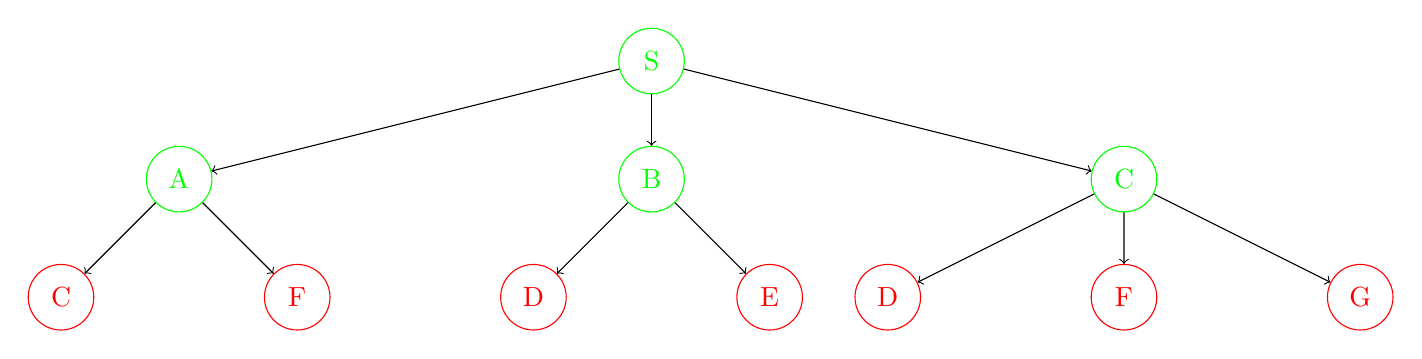
\begin{tikzpicture}[
            ->, 
            level/.style={level distance=1.5cm},
            level 1/.style={sibling distance=6cm},
            level 2/.style={sibling distance=3cm},
            level 3/.style={sibling distance=1.5cm}
        ]
            \node[node_expanded] {S} 
                child { node[node_expanded]{A} 
                    child { node[node_non_expanded]{C} }
                    child { node[node_non_expanded]{F} } 
                }
                child { node[node_expanded]{B}
                    child { node[node_non_expanded]{D} }
                    child { node[node_non_expanded]{E} }
                }
                child { node[node_expanded]{C}
                    child { node[node_non_expanded]{D} }
                    child { node[node_non_expanded]{F} }
                    child { node[node_non_expanded]{G} }
                }
            ;
        \end{tikzpicture}
    \end{center}
    \pagebreak
    \qquad \textit{Step 5.} Now we try to expand the node C. Since C is already expanded, we will not expand it again and we reach the end of a branch.
    \smallskip
    \begin{center}
        \begin{tikzpicture}[
        ->, 
            level/.style={level distance=1.5cm},
            level 1/.style={sibling distance=6cm},
            level 2/.style={sibling distance=3cm},
            level 3/.style={sibling distance=1.5cm}
        ]
            \node[node_expanded] {S} 
                child { node[node_expanded]{A} 
                    child { node[node_expanded]{C} 
                        child { node[node_leaf]{Z} }
                    }
                    child { node[node_non_expanded]{F} } 
                }
                child { node[node_expanded]{B}
                    child { node[node_non_expanded]{D} }
                    child { node[node_non_expanded]{E} }
                }
                child { node[node_expanded]{C}
                    child { node[node_non_expanded]{D} }
                    child { node[node_non_expanded]{F} }
                    child { node[node_non_expanded]{G} }
                }
            ;
        \end{tikzpicture}
    \end{center}
    \medskip
    \qquad \textit{Step 6.} We expand the node F. Since the children of F are the nodes A and C, and they both have been visited, we will not write them again. So F also results in an end of a branch.
    \smallskip
    \begin{center}
        \begin{tikzpicture}[
            ->, 
            level/.style={level distance=1.5cm},
            level 1/.style={sibling distance=6cm},
            level 2/.style={sibling distance=3cm},
            level 3/.style={sibling distance=1.5cm}
        ]
            \node[node_expanded] {S} 
                child { node[node_expanded]{A} 
                    child { node[node_expanded]{C} 
                        child { node[node_leaf]{Z} }
                    }
                    child { node[node_expanded]{F}
                        child { node[node_leaf]{Z} }
                    } 
                }
                child { node[node_expanded]{B}
                    child { node[node_non_expanded]{D}}
                    child { node[node_non_expanded]{E}}
                }
                child { node[node_expanded]{C}
                    child{ node[node_non_expanded]{D}}
                    child{ node[node_non_expanded]{F}}
                    child{ node[node_non_expanded]{G}}
                }
            ;
        \end{tikzpicture}
    \end{center}
    \medskip
    \qquad \textit{Step 7.} We expand the node D. Two of the children of D, namely C and B, have been visited, we will not write them again.
    \smallskip
    \begin{center}
        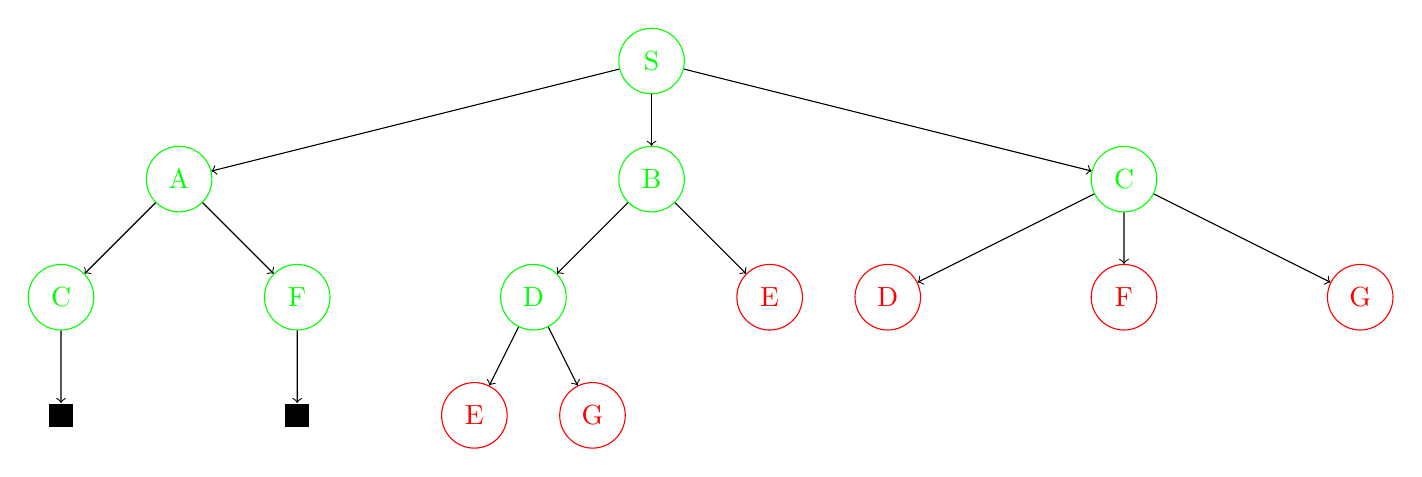
\begin{tikzpicture}[
            ->, 
            level/.style={level distance=1.5cm},
            level 1/.style={sibling distance=6cm},
            level 2/.style={sibling distance=3cm},
            level 3/.style={sibling distance=1.5cm}
        ]
            \node[node_expanded] {S} 
                child { node[node_expanded]{A} 
                    child { node[node_expanded]{C} 
                        child { node[node_leaf]{Z} }
                    }
                    child {  node[node_expanded]{F}
                        child { node[node_leaf]{Z} }
                    } 
                }
                child { node[node_expanded]{B}
                    child { node[node_expanded]{D}
                        child { node[node_non_expanded]{E} }
                        child { node[node_non_expanded]{G} }
                    }
                    child { node[node_non_expanded]{E} }
                }
                child { node[node_expanded]{C}
                    child { node[node_non_expanded]{D} }
                    child { node[node_non_expanded]{F} }
                    child { node[node_non_expanded]{G} }
                }
            ;
        \end{tikzpicture}
    \end{center}
    \pagebreak
    \qquad \textit{Step 8.} We expand the node E. Two of the children of E, namely B and D, have been visited, we will not write them again.
    \smallskip
    \begin{center}
        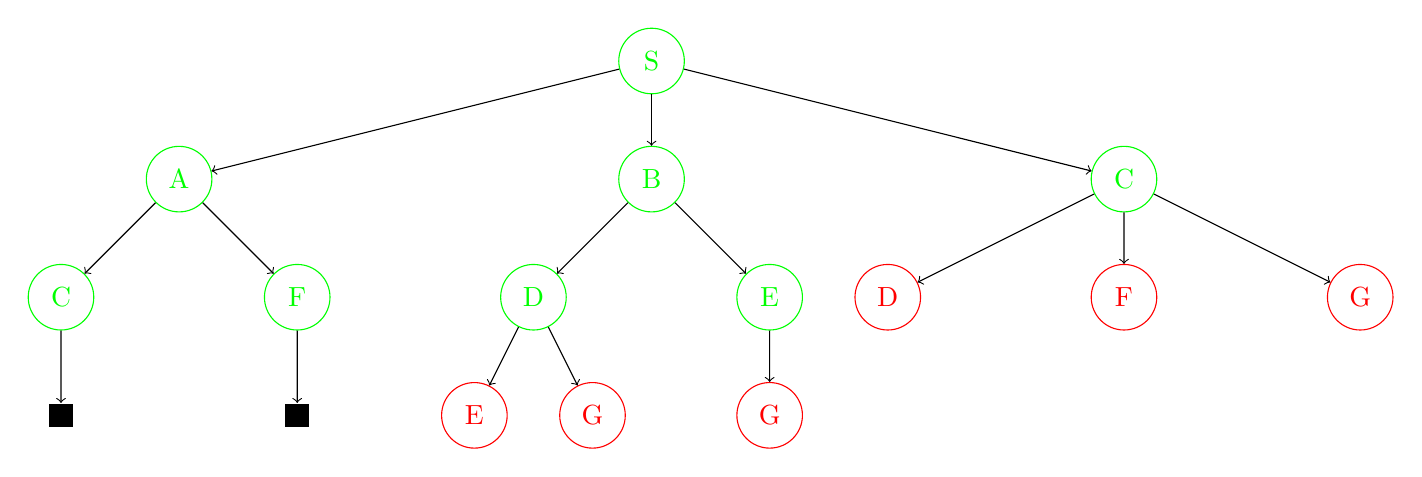
\begin{tikzpicture}[
            ->, 
            level/.style={level distance=1.5cm},
            level 1/.style={sibling distance=6cm},
            level 2/.style={sibling distance=3cm},
            level 3/.style={sibling distance=1.5cm}
        ]
            \node[node_expanded] {S} 
                child { node[node_expanded]{A} 
                    child { node[node_expanded]{C} 
                        child { node[node_leaf]{Z} }
                    }
                    child { node[node_expanded]{F}
                        child { node[node_leaf]{Z} }
                    }
                }
                child { node[node_expanded]{B}
                    child { node[node_expanded]{D}
                        child { node[node_non_expanded]{E} }
                        child { node[node_non_expanded]{G} }
                    }
                    child { node[node_expanded]{E}
                        child { node[node_non_expanded]{G} }
                    }
                }
                child { node[node_expanded]{C}
                    child{ node[node_non_expanded]{D} }
                    child{ node[node_non_expanded]{F} }
                    child{ node[node_non_expanded]{G} }
                }
            ;
        \end{tikzpicture}
    \end{center}
    \medskip
    \qquad \textit{Step 9.} We try to expand the node D. It has been expanded before, so it results in an end.
    \smallskip
    \begin{center}
        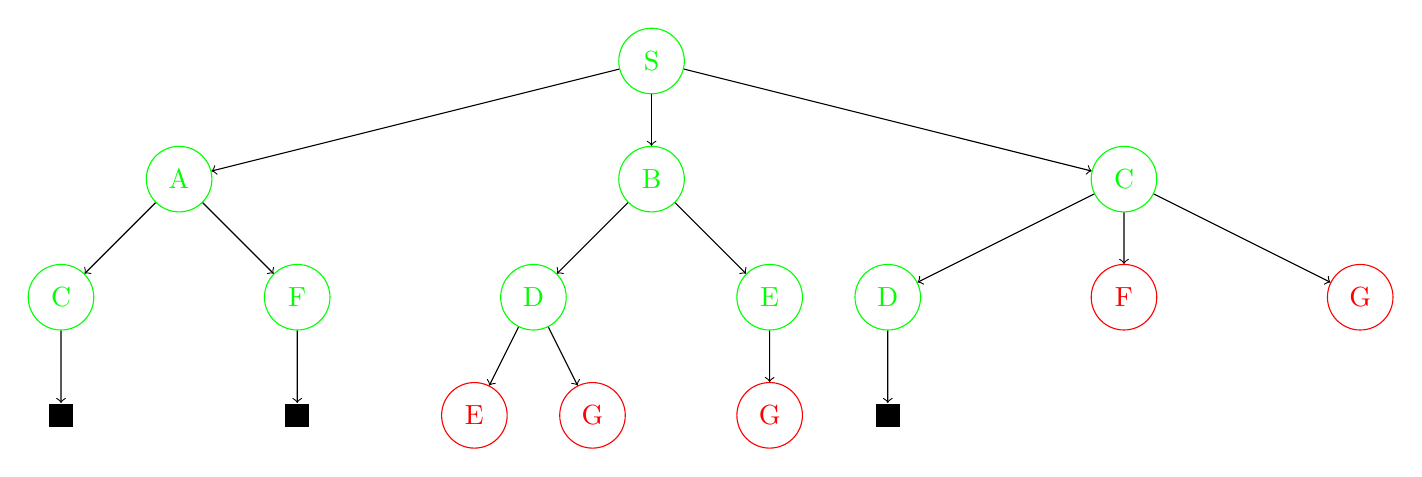
\begin{tikzpicture}[
            ->, 
            level/.style={level distance=1.5cm},
            level 1/.style={sibling distance=6cm},
            level 2/.style={sibling distance=3cm},
            level 3/.style={sibling distance=1.5cm}
        ]
            \node[node_expanded] {S} 
                child { node[node_expanded]{A} 
                    child { node[node_expanded]{C} 
                        child { node[node_leaf]{Z} }
                    }
                    child { node[node_expanded]{F}
                        child { node[node_leaf]{Z} }
                    } 
                }
                child { node[node_expanded]{B}
                    child { node[node_expanded]{D}
                        child { node[node_non_expanded]{E} }
                        child { node[node_non_expanded]{G} }
                    }
                    child { node[node_expanded]{E}
                        child { node[node_non_expanded]{G} }
                    }
                }
                child { node[node_expanded]{C}
                    child { node[node_expanded]{D}
                        child { node[node_leaf]{Z} }
                    }
                    child { node[node_non_expanded]{F}}
                    child { node[node_non_expanded]{G}}
                }
            ;
        \end{tikzpicture}
    \end{center}
    \medskip
    \qquad \textit{Step 10.} We try to expand the node F. It has been expanded before, so no need to expand it again. So it results in an end.
    \smallskip
    \begin{center}
        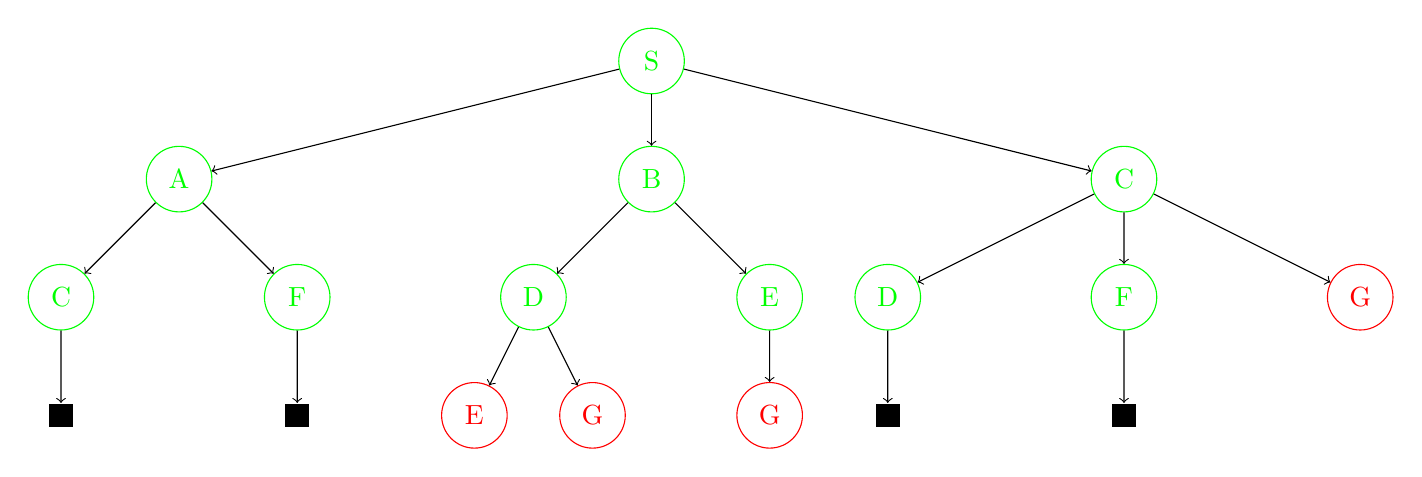
\begin{tikzpicture}[
            ->, 
            level/.style={level distance=1.5cm},
            level 1/.style={sibling distance=6cm},
            level 2/.style={sibling distance=3cm},
            level 3/.style={sibling distance=1.5cm}
        ]
            \node[node_expanded] {S} 
                child { node[node_expanded]{A} 
                    child { node[node_expanded]{C} 
                        child { node[node_leaf]{Z} }
                    }
                    child { node[node_expanded]{F}
                        child { node[node_leaf]{Z} }
                    }
                }
                child { node[node_expanded]{B}
                    child { node[node_expanded]{D}
                        child { node[node_non_expanded]{E} }
                        child { node[node_non_expanded]{G} }
                    }
                    child { node[node_expanded]{E}
                        child { node[node_non_expanded]{G} }
                    }
                }
                child { node[node_expanded]{C}
                    child { node[node_expanded]{D}
                        child { node[node_leaf]{Z} }
                    }
                    child { node[node_expanded]{F}
                        child { node[node_leaf]{Z} }
                    }
                    child { node[node_non_expanded]{G}}
                }
            ;
        \end{tikzpicture}
    \end{center}
    \pagebreak
    \qquad \textit{Step 11.} We try to expand the node G. Since G is the end goal, the search is over. The path obtained from breadth-first search is show by the cyan line.
    \smallskip
    \begin{center}
        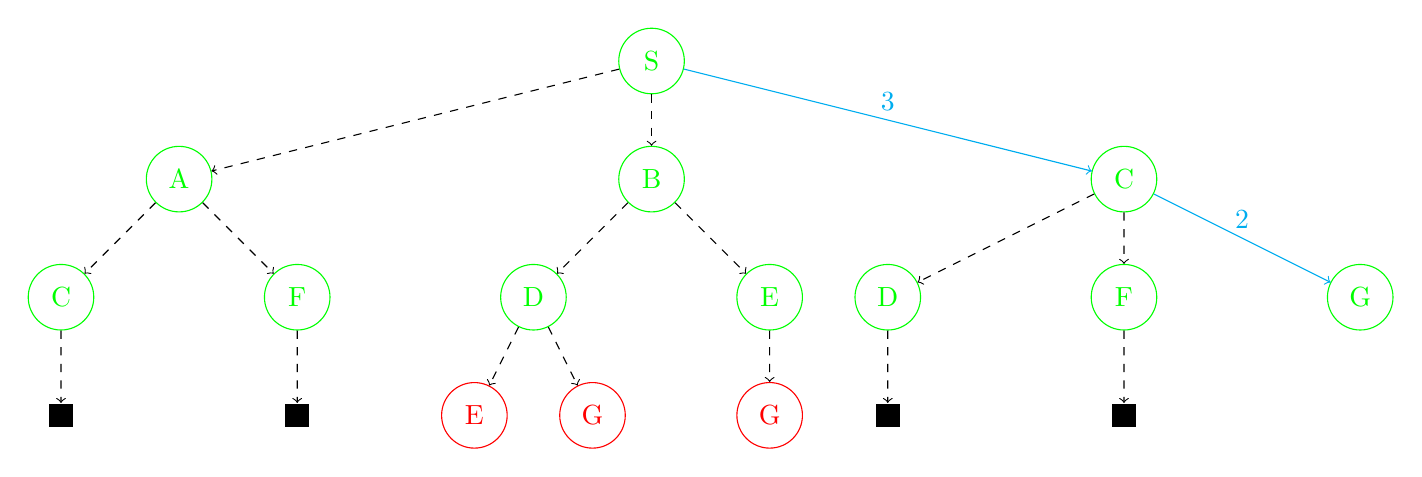
\begin{tikzpicture}[
            ->, 
            level/.style={level distance=1.5cm},
            level 1/.style={sibling distance=6cm},
            level 2/.style={sibling distance=3cm},
            level 3/.style={sibling distance=1.5cm},
            every node/.style={solid}
        ]
            \node[node_expanded] {S} 
                child { node[node_expanded]{A} edge from parent [black, dashed]
                    child { node[node_expanded]{C} edge from parent [black, dashed]
                        child { node[node_leaf]{Z} edge from parent [black, dashed] 
                        }
                    }
                    child { node[node_expanded]{F} edge from parent [black, dashed]
                        child { node[node_leaf]{Z} edge from parent [black, dashed] 
                        }
                    }
                }
                child { node[node_expanded]{B} edge from parent [black, dashed]
                    child { node[node_expanded]{D} edge from parent [black, dashed]
                        child { node[node_non_expanded]{E} edge from parent [black, dashed]
                        }
                        child { node[node_non_expanded]{G} edge from parent [black, dashed]
                        }
                    }
                    child { node[node_expanded]{E} edge from parent [black, dashed]
                        child { node[node_non_expanded]{G} edge from parent [black, dashed]}
                    }
                }
                child { node[node_expanded]{C} edge from parent [cyan]
                    child { node[node_expanded]{D} edge from parent [black, dashed]
                        child { node[node_leaf]{Z} edge from parent [black, dashed]}
                    }
                    child { node[node_expanded]{F} edge from parent [black, dashed]
                        child { node[node_leaf]{Z} edge from parent [black, dashed] 
                        }
                    }
                    child { node[node_expanded]{G} edge from parent [cyan] edge from parent node[above] {2}}
                edge from parent node[above]{3}};
        \end{tikzpicture}
        \medskip
        $$ \Rightarrow Cost = 5 $$
    \end{center}
    \pagebreak
    \subsection{Depth-first Search}
    \medskip
    \qquad \textit{Step 1.} We start expanding from the node S.
    \smallskip
    \begin{center}
        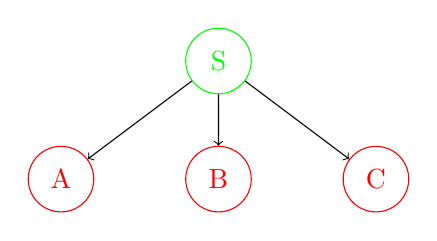
\begin{tikzpicture}[
            ->, 
            level/.style={sibling distance=2cm, level distance=1.5cm}
        ]
            \node[node_expanded] {S} 
                child { node[node_non_expanded]{A} }
                child { node[node_non_expanded]{B} }
                child { node[node_non_expanded]{C} }
            ;
        \end{tikzpicture}
    \end{center}
    \medskip
    \qquad \textit{Step 2.} We expand the node A, since it comes alphabetically before B and C. Since the node S is already expanded, we will not write it again.
    \smallskip
    \begin{center}
        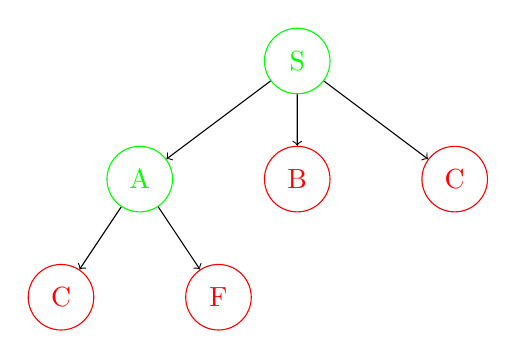
\begin{tikzpicture}[
            ->, 
            level/.style={sibling distance=2cm, level distance=1.5cm}
        ]
            \node[node_expanded] {S} 
                child { node[node_expanded]{A} 
                        child { node[node_non_expanded]{C} }
                        child { node[node_non_expanded]{F} } 
                }
                child { node[node_non_expanded]{B} }
                child { node[node_non_expanded]{C} }
            ;
        \end{tikzpicture}
    \end{center}
    \medskip
    \qquad \textit{Step 3.} We now expand the node C, since it comes alphabetically before node F.
    \smallskip
    \begin{center}
        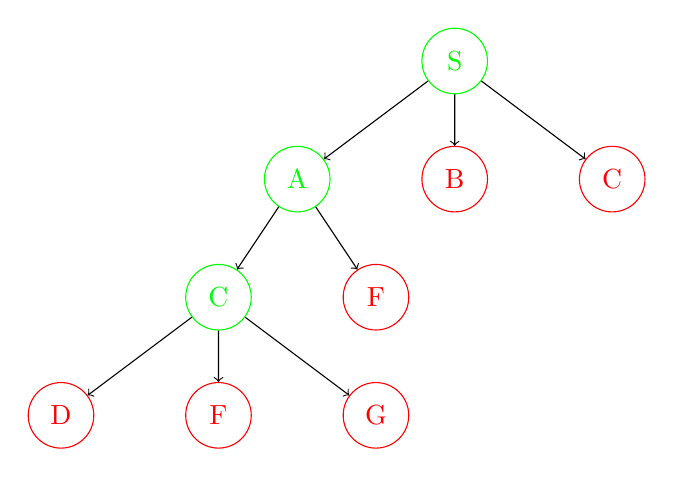
\begin{tikzpicture}[
            ->, 
            level/.style={sibling distance=2cm, level distance=1.5cm}
        ]
            \node[node_expanded] {S} 
                child { node[node_expanded]{A} 
                        child { node[node_expanded]{C} 
                            child { node[node_non_expanded]{D} }
                            child { node[node_non_expanded]{F} }
                            child { node[node_non_expanded]{G} }
                        }
                        child { node[node_non_expanded]{F} } 
                }
                child { node[node_non_expanded]{B} }
                child { node[node_non_expanded]{C} }
            ;
        \end{tikzpicture}
    \end{center}
    \medskip
    \qquad \textit{Step 4.} We expand the node D, since it comes alphabetically before node F and node G.
    \smallskip
    \begin{center}
        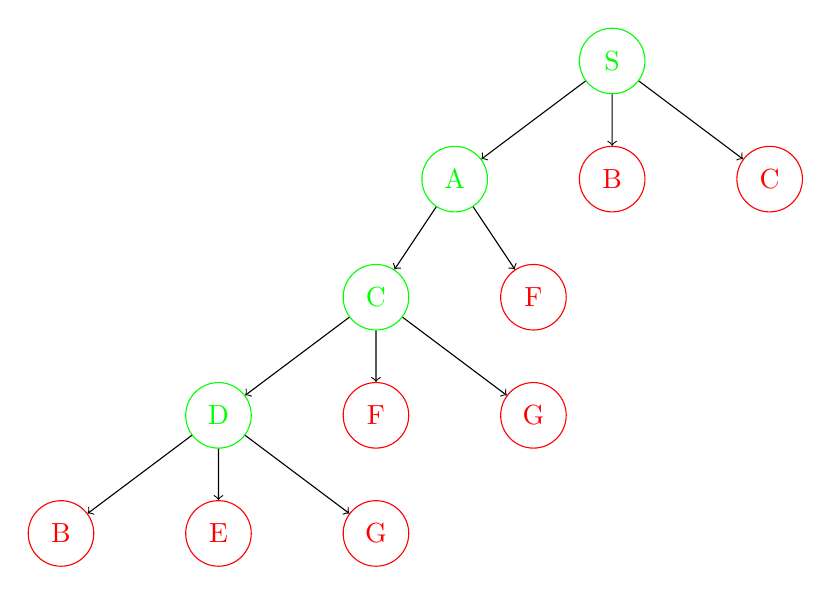
\begin{tikzpicture}[
            ->, 
            level/.style={sibling distance=2cm, level distance=1.5cm}
        ]
            \node[node_expanded] {S} 
                child { node[node_expanded]{A} 
                        child { node[node_expanded]{C} 
                            child { node[node_expanded]{D}
                                child { node[node_non_expanded]{B} }
                                child { node[node_non_expanded]{E} }
                                child { node[node_non_expanded]{G} }
                            }
                            child { node[node_non_expanded]{F} }
                            child { node[node_non_expanded]{G} }
                        }
                        child { node[node_non_expanded]{F} } 
                }
                child { node[node_non_expanded]{B} }
                child { node[node_non_expanded]{C} }
            ;
        \end{tikzpicture}
    \end{center}
    \medskip
    \qquad \textit{Step 5.} We expand the node B, since it comes alphabetically before node E and node G.
    \smallskip
    \begin{center}
        \begin{tikzpicture}[
            ->, 
            level/.style={sibling distance=2cm, level distance=1.5cm}
        ]
            \node[node_expanded] {S} 
                child { node[node_expanded]{A} 
                        child { node[node_expanded]{C} 
                            child { node[node_expanded]{D}
                                child { node[node_expanded]{B}
                                    child { node [node_non_expanded]{E} }
                                }
                                child { node[node_non_expanded]{E} }
                                child { node[node_non_expanded]{G} }
                            }
                            child { node[node_non_expanded]{F} }
                            child { node[node_non_expanded]{G} }
                        }
                        child { node[node_non_expanded]{F} } 
                }
                child { node[node_non_expanded]{B} }
                child { node[node_non_expanded]{C} }
            ;
        \end{tikzpicture}
    \end{center}
    \medskip
    \qquad \textit{Step 6.} We expand the node E.
    \smallskip
    \begin{center}
        \begin{tikzpicture}[
            ->, 
            level/.style={sibling distance=2cm, level distance=1.5cm}
        ]
            \node[node_expanded] {S} 
                child { node[node_expanded]{A} 
                        child { node[node_expanded]{C} 
                            child { node[node_expanded]{D}
                                child { node[node_expanded]{B}
                                    child { node[node_expanded]{E}
                                        child { node[node_non_expanded]{G} }
                                    }
                                }
                                child { node[node_non_expanded]{E} }
                                child { node[node_non_expanded]{G} }
                            }
                            child { node[node_non_expanded]{F} }
                            child { node[node_non_expanded]{G} }
                        }
                        child { node[node_non_expanded]{F} } 
                }
                child { node[node_non_expanded]{B} }
                child { node[node_non_expanded]{C} }
            ;
        \end{tikzpicture}
    \end{center}
    \pagebreak
    \qquad \textit{Step 7.} We have reached the end goal G, thus the search is over. The path returned by the depth-first search is shown by the cyan line.
    \smallskip
    \begin{center}
        \begin{tikzpicture}[
            ->, 
            level/.style={sibling distance=2cm, level distance=1.5cm},
            every node/.style={solid}
        ]
            \node[node_expanded] {S} 
                child { node[node_expanded]{A} edge from parent [cyan]
                        child { node[node_expanded]{C} edge from parent [cyan]
                            child { node[node_expanded]{D} edge from parent [cyan]
                                child { node[node_expanded]{B} edge from parent [cyan]
                                    child { node [node_expanded]{E} edge from parent [cyan]
                                        child { node [node_expanded]{G} edge from parent [cyan] edge from parent node[left]{5}
                                        }
                                    edge from parent node[left]{2}
                                    }
                                edge from parent node[left]{3}
                                }
                                child { node[node_non_expanded]{E} edge from parent [black, dashed]}
                                child { node[node_non_expanded]{G} edge from parent [black, dashed]}
                            edge from parent node[left]{5}
                            }
                            child { node[node_non_expanded]{F} edge from parent [black, dashed]}
                            child { node[node_non_expanded]{G} edge from parent [black, dashed]}
                        edge from parent node[left]{2}
                        }
                        child { node[node_non_expanded]{F} edge from parent [black, dashed]} 
                edge from parent node[left]{2}
            }
                child{ node[node_non_expanded]{B} edge from parent [black, dashed]}
                child{ node[node_non_expanded]{C} edge from parent [black, dashed]};
        \end{tikzpicture}
        $$ \Rightarrow Cost = 19 $$
    \end{center}
    \pagebreak
    \subsection{Iterative Deepening Search}
    \medskip
    \subsubsection*{$\text{Depth Bound} = 0$}
    Since the node S is the starting node and it is not our goal, thus we need to increment the depth bound.
    \bigskip
    \subsubsection*{$\text{Depth Bound} = 1$}
    \qquad \textit{Step 1.} We expand the node S.
    \smallskip
    \begin{center}
        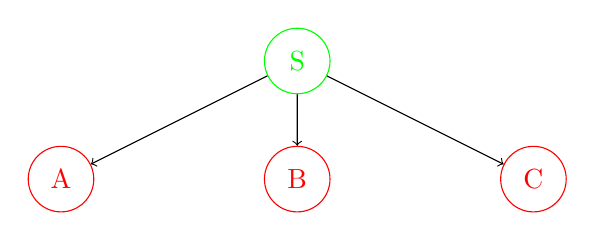
\begin{tikzpicture}[
            ->, 
            level/.style={level distance=1.5cm},
            level 1/.style={sibling distance=3cm},
            level 2/.style={sibling distance=1.5cm}
        ]
            \node[node_expanded] {S} 
                child { node[node_non_expanded]{A} }
                child { node[node_non_expanded]{B} }
                child { node[node_non_expanded]{C} }
            ;
        \end{tikzpicture}
    \end{center}
    \medskip
    \qquad \textit{Step 2.} We now try to expand the node A, since it comes alphabetically before nodes B and C. Since our maximum depth bound is 1, so we cannot expand A.
    \smallskip
    \begin{center}
        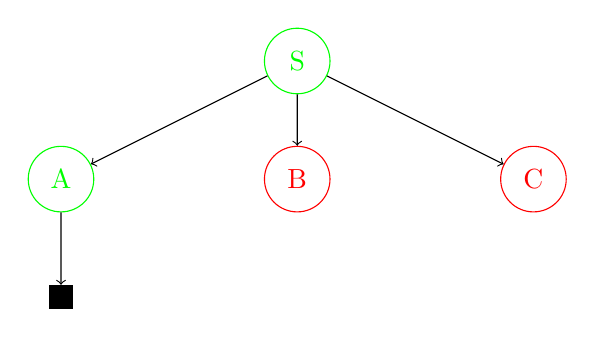
\begin{tikzpicture}[
            ->, 
            level/.style={level distance=1.5cm},
            level 1/.style={sibling distance=3cm},
            level 2/.style={sibling distance=1.5cm}
        ]
            \node[node_expanded] {S} 
                child { node[node_expanded]{A} 
                    child { node[node_leaf]{Z} }
                }
                child { node[node_non_expanded]{B} }
                child { node[node_non_expanded]{C} }
            ;
        \end{tikzpicture}
    \end{center}
    \medskip
    \qquad \textit{Step 3.} We now try to expand the node B. Since our maximum depth bound is 1, so we cannot expand node B neither.
    \smallskip
    \begin{center}
        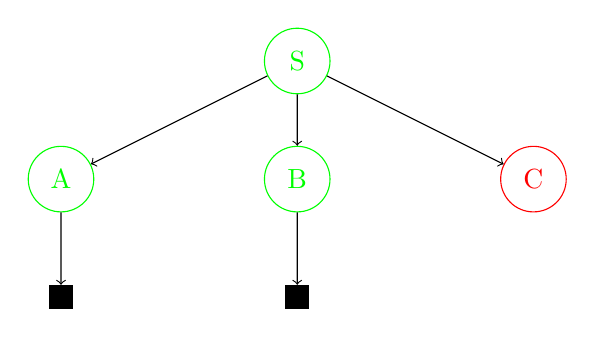
\begin{tikzpicture}[
            ->, 
            level/.style={level distance=1.5cm},
            level 1/.style={sibling distance=3cm},
            level 2/.style={sibling distance=1.5cm}
        ]
            \node[node_expanded] {S} 
                child { node[node_expanded]{A} 
                    child { node[node_leaf]{Z} }
                }
                child { node[node_expanded]{B}
                    child { node[node_leaf]{Z} }
                }
                child { node[node_non_expanded]{C} }
            ;
        \end{tikzpicture}
    \end{center}
    \medskip
    \qquad \textit{Step 4.} We now try to expand the node C. Since our maximum depth bound is 1, so we cannot expand node C neither. We did not reach the goal node, so the depth must be incremented.
    \smallskip
    \begin{center}
        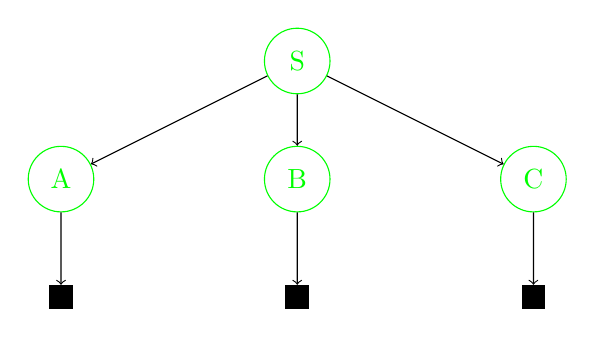
\begin{tikzpicture}[
            ->, 
            level/.style={level distance=1.5cm},
            level 1/.style={sibling distance=3cm},
            level 2/.style={sibling distance=1.5cm}
        ]
            \node[node_expanded] {S} 
                child { node[node_expanded]{A} 
                    child { node[node_leaf]{Z} }
                }
                child { node[node_expanded]{B}
                    child { node[node_leaf]{Z} }
                }
                child { node[node_expanded]{C} 
                    child { node[node_leaf]{Z} }
                }
            ;
        \end{tikzpicture}
    \end{center}
    \subsubsection*{$\text{Depth Bound} = 2$}
    \qquad \textit{Step 1.} We expand the node S.
    \smallskip
    \begin{center}
        \begin{tikzpicture}[
            ->, 
            level/.style={level distance=1.5cm},
            level 1/.style={sibling distance=6cm},
            level 2/.style={sibling distance=3cm},
            level 3/.style={sibling distance=1.5cm}
        ]
            \node[node_expanded] {S} 
                child { node[node_non_expanded]{A} }
                child { node[node_non_expanded]{B} }
                child { node[node_non_expanded]{C} }
            ;
        \end{tikzpicture}
    \end{center}
    \medskip
    \qquad \textit{Step 2.} We now try to expand the node A, since it comes alphabetically before nodes B and C. Node S has already been expanded so no need to write it again.
    \smallskip
    \begin{center}
        \begin{tikzpicture}[
            ->, 
            level/.style={level distance=1.5cm},
            level 1/.style={sibling distance=6cm},
            level 2/.style={sibling distance=3cm},
            level 3/.style={sibling distance=1.5cm}
        ]
            \node[node_expanded] {S} 
                child { node[node_expanded]{A} 
                    child { node[node_non_expanded]{C} }
                    child { node[node_non_expanded]{F} } 
                }
                child { node[node_non_expanded]{B} }
                child { node[node_non_expanded]{C} }
            ;
        \end{tikzpicture}
    \end{center}
    \medskip
    \qquad \textit{Step 3.} We now try to expand the node C, since it comes alphabetically before node F. We have reached the maximum depth, and C is not our goal, so we fail to expand C and we reach end of the branch.
    \smallskip
    \begin{center}
        \begin{tikzpicture}[
            ->, 
            level/.style={level distance=1.5cm},
            level 1/.style={sibling distance=6cm},
            level 2/.style={sibling distance=3cm},
            level 3/.style={sibling distance=1.5cm}
        ]
            \node[node_expanded] {S} 
                child { node[node_expanded]{A} 
                    child { node[node_expanded]{C} 
                        child { node[node_leaf]{Z} }
                    }
                    child { node[node_non_expanded]{F} } 
                }
                child { node[node_non_expanded]{B} }
                child { node[node_non_expanded]{C} }
            ;
        \end{tikzpicture}
    \end{center}
    \medskip
    \qquad \textit{Step 4.} We now try to expand the node F. We have reached the maximum depth, and F is not our goal, so we fail to expand F and we reach end of the branch.
    \smallskip
    \begin{center}
        \begin{tikzpicture}[
            ->, 
            level/.style={level distance=1.5cm},
            level 1/.style={sibling distance=6cm},
            level 2/.style={sibling distance=3cm},
            level 3/.style={sibling distance=1.5cm}
        ]
            \node[node_expanded] {S} 
                child { node[node_expanded]{A} 
                    child { node[node_expanded]{C} 
                        child { node[node_leaf]{Z} }
                    }
                    child { node[node_expanded]{F} 
                        child { node[node_leaf]{Z} }
                    } 
                }
                child { node[node_non_expanded]{B} }
                child { node[node_non_expanded]{C} }
            ;
        \end{tikzpicture}
    \end{center}
    \pagebreak
    \qquad \textit{Step 5.} We now expand the node B.
    \smallskip
    \begin{center}
        \begin{tikzpicture}[
            ->, 
            level/.style={level distance=1.5cm},
            level 1/.style={sibling distance=6cm},
            level 2/.style={sibling distance=3cm},
            level 3/.style={sibling distance=1.5cm}
        ]
            \node[node_expanded] {S} 
                child { node[node_expanded]{A} 
                    child { node[node_expanded]{C} 
                        child { node[node_leaf]{Z} }
                    }
                    child { node[node_expanded]{F} 
                        child { node[node_leaf]{Z} }
                    } 
                }
                child { node[node_expanded]{B}
                    child { node[node_non_expanded]{D} }
                    child { node[node_non_expanded]{E} }
                }
                child { node[node_non_expanded]{C} }
            ;
        \end{tikzpicture}
    \end{center}
    \medskip
    \qquad \textit{Step 6.} We try to expand D. We have reached the maximum depth, and D is not our goal, so we fail to expand D and we reach end of the branch.
    \smallskip
    \begin{center}
        \begin{tikzpicture}[
            ->, 
            level/.style={level distance=1.5cm},
            level 1/.style={sibling distance=6cm},
            level 2/.style={sibling distance=3cm},
            level 3/.style={sibling distance=1.5cm}
        ]
            \node[node_expanded] {S} 
                child { node[node_expanded]{A} 
                    child { node[node_expanded]{C} 
                        child { node[node_leaf]{Z} }
                    }
                    child { node[node_expanded]{F} 
                        child { node[node_leaf]{Z} }
                    } 
                }
                child { node[node_expanded]{B}
                    child { node[node_expanded]{D} 
                        child { node[node_leaf]{Z} }
                    }
                    child { node[node_non_expanded]{E} }
                }
                child { node[node_non_expanded]{C} }
            ;
        \end{tikzpicture}
    \end{center}
    \medskip
    \qquad \textit{Step 7.} We try to expand E. We have reached the maximum depth, and E is not our goal, so we fail to expand E and we reach end of the branch.
    \smallskip
    \begin{center}
        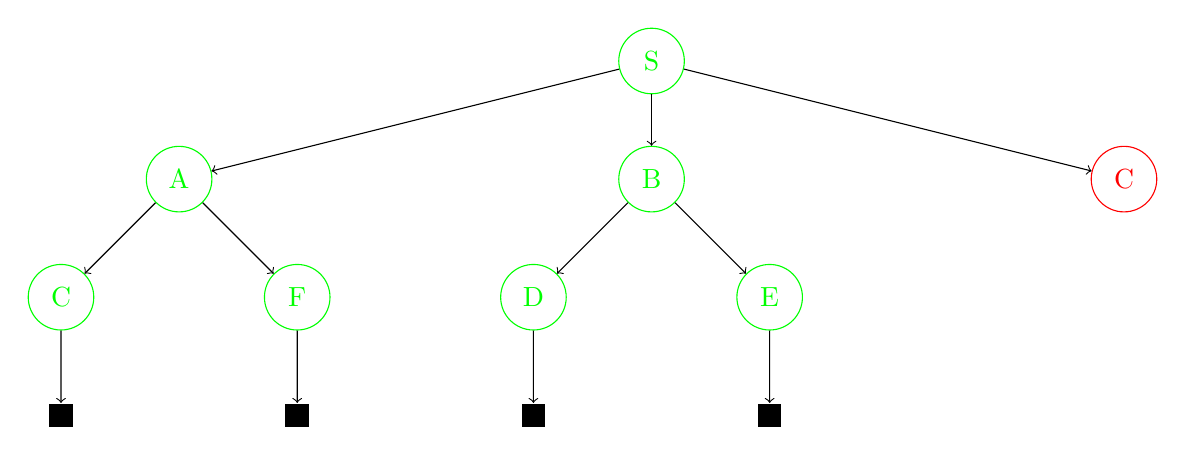
\begin{tikzpicture}[
            ->, 
            level/.style={level distance=1.5cm},
            level 1/.style={sibling distance=6cm},
            level 2/.style={sibling distance=3cm},
            level 3/.style={sibling distance=1.5cm}
        ]
            \node[node_expanded] {S} 
                child { node[node_expanded]{A} 
                    child { node[node_expanded]{C} 
                        child { node[node_leaf]{Z} }
                    }
                    child { node[node_expanded]{F} 
                        child { node[node_leaf]{Z} }
                    } 
                }
                child { node[node_expanded]{B}
                    child { node[node_expanded]{D} 
                        child { node[node_leaf]{Z} }
                    }
                    child { node[node_expanded]{E} 
                        child { node[node_leaf]{Z} }
                    }
                }
                child { node[node_non_expanded]{C} }
            ;
        \end{tikzpicture}
    \end{center}
    \medskip
    \qquad \textit{Step 8.} We try to expand C. Since C was already expanded, we cannot expand it again.
    \smallskip
    \begin{center}
        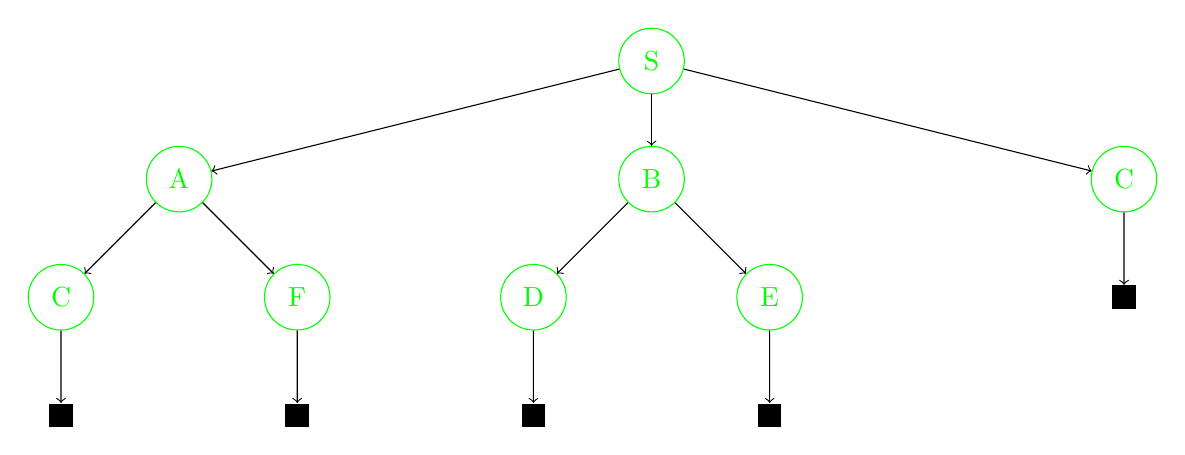
\begin{tikzpicture}[
            ->, 
            level/.style={level distance=1.5cm},
            level 1/.style={sibling distance=6cm},
            level 2/.style={sibling distance=3cm},
            level 3/.style={sibling distance=1.5cm}
        ]
            \node[node_expanded] {S} 
                child { node[node_expanded]{A} 
                    child { node[node_expanded]{C} 
                        child { node[node_leaf]{Z} }
                    }
                    child { node[node_expanded]{F} 
                        child { node[node_leaf]{Z} }
                    } 
                }
                child { node[node_expanded]{B}
                    child { node[node_expanded]{D} 
                        child { node[node_leaf]{Z} }
                    }
                    child { node[node_expanded]{E} 
                        child { node[node_leaf]{Z} }
                    }
                }
                child { node[node_expanded]{C} 
                    child { node[node_leaf]{Z} }
                }
            ;
        \end{tikzpicture}
    \end{center}
    \subsubsection*{$\text{Depth Bound} = 3$}
    \qquad \textit{Step 1.} We expand the node S.
    \smallskip
    \begin{center}
        \begin{tikzpicture}[
            ->, 
            level/.style={level distance=1.5cm},
            level 1/.style={sibling distance=6cm},
            level 2/.style={sibling distance=3cm},
            level 3/.style={sibling distance=1.5cm}
        ]
            \node[node_expanded] {S} 
                child { node[node_non_expanded]{A} }
                child { node[node_non_expanded]{B} }
                child { node[node_non_expanded]{C} }
            ;
        \end{tikzpicture}
    \end{center}
    \medskip
    \qquad \textit{Step 2.} We now try to expand the node A, since it comes alphabetically before nodes B and C. Node S has already been expanded so no need to write it again.
    \smallskip
    \begin{center}
        \begin{tikzpicture}[
            ->, 
            level/.style={level distance=1.5cm},
            level 1/.style={sibling distance=6cm},
            level 2/.style={sibling distance=3cm},
            level 3/.style={sibling distance=1.5cm}
        ]
            \node[node_expanded] {S} 
                child { node[node_expanded]{A} 
                    child { node[node_non_expanded]{C} }
                    child { node[node_non_expanded]{F} } 
                }
                child { node[node_non_expanded]{B} }
                child { node[node_non_expanded]{C} }
            ;
        \end{tikzpicture}
    \end{center}
    \medskip
    \qquad \textit{Step 3.} We now try to expand the node C, since it comes alphabetically before node F. 
    \smallskip
    \begin{center}
        \begin{tikzpicture}[
            ->, 
            level/.style={level distance=1.5cm},
            level 1/.style={sibling distance=5.5cm},
            level 2/.style={sibling distance=3cm},
            level 3/.style={sibling distance=1.25cm},
            level 4/.style={sibling distance=7.5mm}
        ]
            \node[node_expanded] {S} 
                child { node[node_expanded]{A} 
                    child { node[node_expanded]{C} 
                        child { node[node_non_expanded]{D} }
                        child { node[node_non_expanded]{F} }
                        child { node[node_non_expanded]{G} }
                    }
                    child { node[node_non_expanded]{F} } 
                }
                child { node[node_non_expanded]{B} }
                child { node[node_non_expanded]{C} }
            ;
        \end{tikzpicture}
    \end{center}
    \medskip
    \qquad \textit{Step 4.} We now try to expand the node D, since it comes alphabetically before nodes F and G. We have reached the maximum depth, so we reach the end of branch. 
    \smallskip
    \begin{center}
        \begin{tikzpicture}[
            ->, 
            level/.style={level distance=1.5cm},
            level 1/.style={sibling distance=5.5cm},
            level 2/.style={sibling distance=3cm},
            level 3/.style={sibling distance=1.25cm},
            level 4/.style={sibling distance=7.5mm}
        ]
            \node[node_expanded] {S} 
                child { node[node_expanded]{A} 
                    child { node[node_expanded]{C} 
                        child { node[node_expanded]{D} 
                            child { node[node_leaf]{Z} }
                        }
                        child { node[node_non_expanded]{F} }
                        child { node[node_non_expanded]{G} }
                    }
                    child { node[node_non_expanded]{F} } 
                }
                child { node[node_non_expanded]{B} }
                child { node[node_non_expanded]{C} }
            ;
        \end{tikzpicture}
    \end{center}
    \medskip
    \qquad \textit{Step 5.} We now try to expand the node F. We have reached the maximum depth, so we reach the end of branch. 
    \smallskip
    \begin{center}
        \begin{tikzpicture}[
            ->, 
            level/.style={level distance=1.5cm},
            level 1/.style={sibling distance=5.5cm},
            level 2/.style={sibling distance=3cm},
            level 3/.style={sibling distance=1.25cm},
            level 4/.style={sibling distance=7.5mm}
        ]
            \node[node_expanded] {S} 
                child { node[node_expanded]{A} 
                    child { node[node_expanded]{C} 
                        child { node[node_expanded]{D} 
                            child { node[node_leaf]{Z} }
                        }
                        child { node[node_expanded]{F} 
                            child { node[node_leaf]{Z} }
                        }
                        child { node[node_non_expanded]{G} }
                    }
                    child { node[node_non_expanded]{F} } 
                }
                child { node[node_non_expanded]{B} }
                child { node[node_non_expanded]{C} }
            ;
        \end{tikzpicture}
    \end{center}
    \medskip
    \qquad \textit{Step 6.} We now try to expand the node G. Since G is our goal, thus the search is over. The path obtained from iterative deepening search is shown by the cyan line.
    \smallskip
    \begin{center}
        \begin{tikzpicture}[
            ->, 
            level/.style={level distance=1.5cm},
            level 1/.style={sibling distance=5.5cm},
            level 2/.style={sibling distance=3cm},
            level 3/.style={sibling distance=1.25cm},
            level 4/.style={sibling distance=7.5mm},
            every node/.style={solid}
        ]
            \node[node_expanded] {S} 
                child { node[node_expanded]{A} edge from parent [cyan]
                    child { node[node_expanded]{C} edge from parent [cyan]
                        child { node[node_expanded]{D} edge from parent [black, dashed]
                            child { node[node_leaf]{Z} edge from parent [black, dashed] }
                        }
                        child { node[node_expanded]{F} edge from parent [black, dashed]
                            child { node[node_leaf]{Z} edge from parent [black, dashed] }
                        }
                        child { node[node_expanded]{G} edge from parent [cyan] edge from parent node[above]{2} }
                    edge from parent node[above]{2} }
                    child { node[node_non_expanded]{F} edge from parent [black, dashed] } 
                edge from parent node[above]{2} }
                child { node[node_non_expanded]{B} edge from parent [black, dashed] }
                child { node[node_non_expanded]{C} edge from parent [black, dashed] }
            ;
        \end{tikzpicture}
        $$ \Rightarrow Cost = 6 $$
    \end{center}
    \pagebreak
    \subsection{Uniform Cost Search}
    \medskip
    \qquad \textit{Step 1.} We start expanding from the node S.
    \smallskip
    \begin{center}
        \begin{tikzpicture}[
            ->, 
            level/.style={level distance=1.5cm},
            level 1/.style={sibling distance=6cm},
            level 2/.style={sibling distance=0.5cm, level distance=1cm},
            level 3/.style={sibling distance=1.5cm}
        ]
            \node[node_expanded] {S} 
                child { node[node_non_expanded]{A} 
                    child { node[node_cost]{2} }
                edge from parent node[above]{2} }
                child { node[node_non_expanded]{B} 
                    child { node[node_cost]{1} }
                edge from parent node[left]{1} }
                child { node[node_non_expanded]{C} 
                    child { node[node_cost]{3} }
                edge from parent node[above]{3} }
            ;
        \end{tikzpicture}
    \end{center}
    \medskip
    \qquad \textit{Step 2.} We now expand node B because it has the minimum cost.
    \smallskip
    \begin{center}
        \begin{tikzpicture}[
            ->, 
            level/.style={level distance=1.5cm},
            level 1/.style={sibling distance=6cm},
            level 2/.style={sibling distance=3cm},
            level 3/.style={sibling distance=1.5cm, level distance=1cm}
        ]
            \node[node_expanded] {S} 
                child { node[node_non_expanded]{A} 
                    child { node[node_cost]{2} }
                edge from parent node[above]{2} }
                child { node[node_expanded]{B} 
                    child { node[node_non_expanded]{D}
                        child { node[node_cost]{4} }
                    edge from parent node[left]{3} }
                    child { node[node_non_expanded]{E} 
                        child { node[node_cost]{3} }
                    edge from parent node[right]{2} }
                edge from parent node[left]{1} }
                child { node[node_non_expanded]{C} 
                    child { node[node_cost]{3} }
                edge from parent node[above]{3} }
            ;
        \end{tikzpicture}
    \end{center}
    \medskip
    \qquad \textit{Step 3.} We now expand node A because it is the cheapest.
    \smallskip
    \begin{center}
        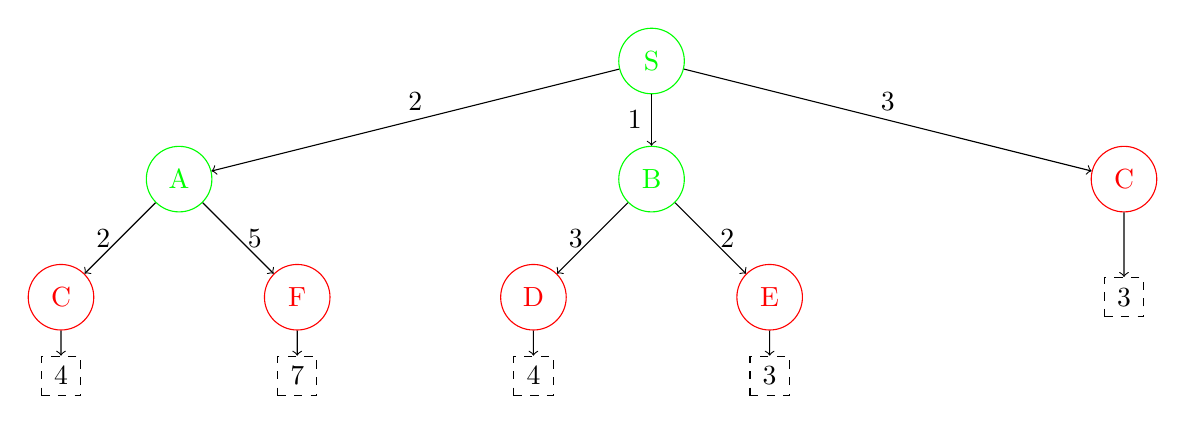
\begin{tikzpicture}[
            ->, 
            level/.style={level distance=1.5cm},
            level 1/.style={sibling distance=6cm},
            level 2/.style={sibling distance=3cm},
            level 3/.style={sibling distance=1.5cm, level distance=1cm}
        ]
            \node[node_expanded] {S} 
                child { node[node_expanded]{A}
                    child { node[node_non_expanded]{C} 
                    child { node[node_cost]{4} }
                    edge from parent node[left]{2} }
                    child { node[node_non_expanded]{F} 
                    child { node[node_cost]{7} }
                    edge from parent node[right]{5} }
                edge from parent node[above]{2} }
                child { node[node_expanded]{B} 
                    child { node[node_non_expanded]{D}
                        child { node[node_cost]{4} }
                    edge from parent node[left]{3} }
                    child { node[node_non_expanded]{E} 
                        child { node[node_cost]{3} }
                    edge from parent node[right]{2} }
                edge from parent node[left]{1} }
                child { node[node_non_expanded]{C} 
                    child { node[node_cost]{3} }
                edge from parent node[above]{3} }
            ;
        \end{tikzpicture}
    \end{center}
    \medskip
    \qquad \textit{Step 4.} We now expand node C since it's the cheapest and it comes alphabetically before node E.
    \smallskip
    \begin{center}
        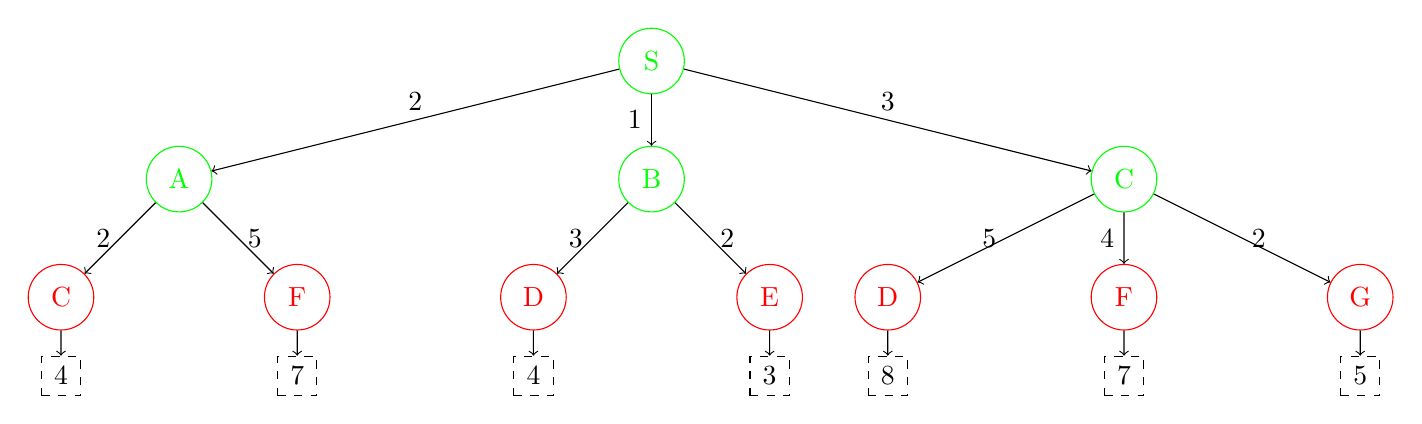
\begin{tikzpicture}[
            ->, 
            level/.style={level distance=1.5cm},
            level 1/.style={sibling distance=6cm},
            level 2/.style={sibling distance=3cm},
            level 3/.style={sibling distance=1.5cm, level distance=1cm}
        ]
            \node[node_expanded] {S} 
                child { node[node_expanded]{A}
                    child { node[node_non_expanded]{C} 
                    child { node[node_cost]{4} }
                    edge from parent node[left]{2} }
                    child { node[node_non_expanded]{F} 
                    child { node[node_cost]{7} }
                    edge from parent node[right]{5} }
                edge from parent node[above]{2} }
                child { node[node_expanded]{B} 
                    child { node[node_non_expanded]{D}
                        child { node[node_cost]{4} }
                    edge from parent node[left]{3} }
                    child { node[node_non_expanded]{E} 
                        child { node[node_cost]{3} }
                    edge from parent node[right]{2} }
                edge from parent node[left]{1} }
                child { node[node_expanded]{C} 
                    child { node[node_non_expanded]{D} 
                    child { node[node_cost]{8} }
                    edge from parent node[left]{5} }
                    child { node[node_non_expanded]{F} 
                    child { node[node_cost]{7} }
                    edge from parent node[left]{4} }
                    child { node[node_non_expanded]{G} 
                    child { node[node_cost]{5} }
                    edge from parent node[right]{2} }
                edge from parent node[above]{3} }
            ;
        \end{tikzpicture}
    \end{center}
    \pagebreak
    \qquad \textit{Step 5.} We now expand node E since it is the cheapest.
    \smallskip
    \begin{center}
        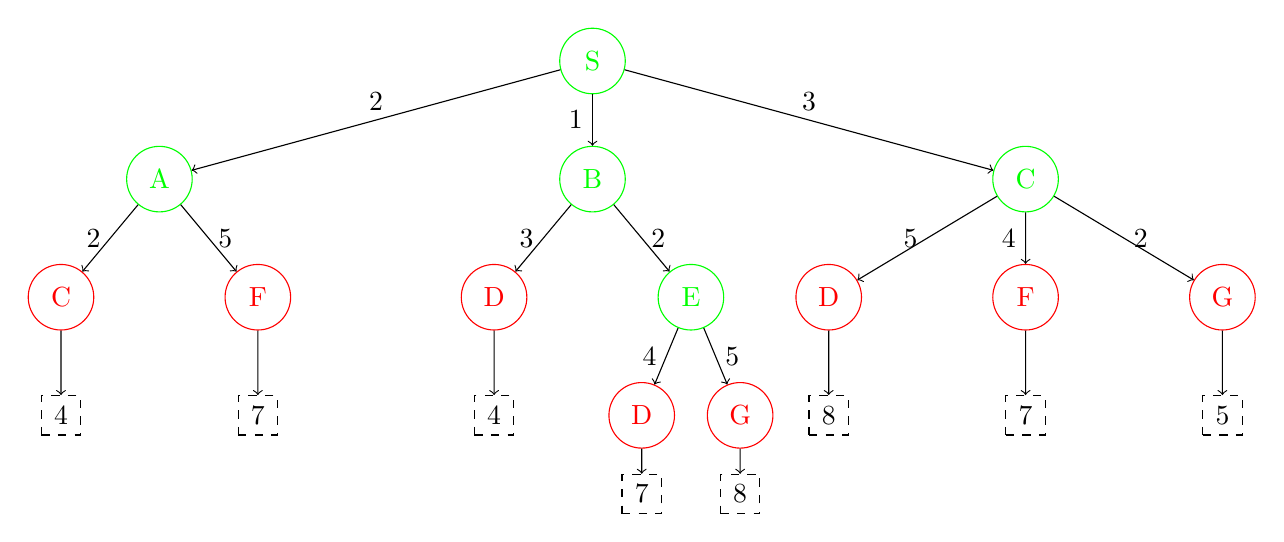
\begin{tikzpicture}[
            ->, 
            level/.style={level distance=1.5cm},
            level 1/.style={sibling distance=5.5cm},
            level 2/.style={sibling distance=2.5cm},
            level 3/.style={sibling distance=1.25cm},
            level 4/.style={sibling distance=1.75cm, level distance=1cm}
        ]
            \node[node_expanded] {S} 
                child { node[node_expanded]{A}
                    child { node[node_non_expanded]{C} 
                    child { node[node_cost]{4} }
                    edge from parent node[left]{2} }
                    child { node[node_non_expanded]{F} 
                    child { node[node_cost]{7} }
                    edge from parent node[right]{5} }
                edge from parent node[above]{2} }
                child { node[node_expanded]{B} 
                    child { node[node_non_expanded]{D}
                        child { node[node_cost]{4} }
                    edge from parent node[left]{3} }
                    child { node[node_expanded]{E} 
                        child { node[node_non_expanded]{D} 
                            child { node[node_cost]{7} }
                        edge from parent node[left]{4} }
                        child { node[node_non_expanded]{G} 
                            child { node[node_cost]{8} }
                        edge from parent node[right]{5} }
                    edge from parent node[right]{2} }
                edge from parent node[left]{1} }
                child { node[node_expanded]{C} 
                    child { node[node_non_expanded]{D} 
                    child { node[node_cost]{8} }
                    edge from parent node[left]{5} }
                    child { node[node_non_expanded]{F} 
                    child { node[node_cost]{7} }
                    edge from parent node[left]{4} }
                    child { node[node_non_expanded]{G} 
                    child { node[node_cost]{5} }
                    edge from parent node[right]{2} }
                edge from parent node[above]{3} }
            ;
        \end{tikzpicture}
    \end{center}
    \medskip
    \qquad \textit{Step 6.} We now try to expand node C since it is the cheapest and comes before node D. But we have already expanded C. So we reach the end of the branch    \smallskip
    \begin{center}
        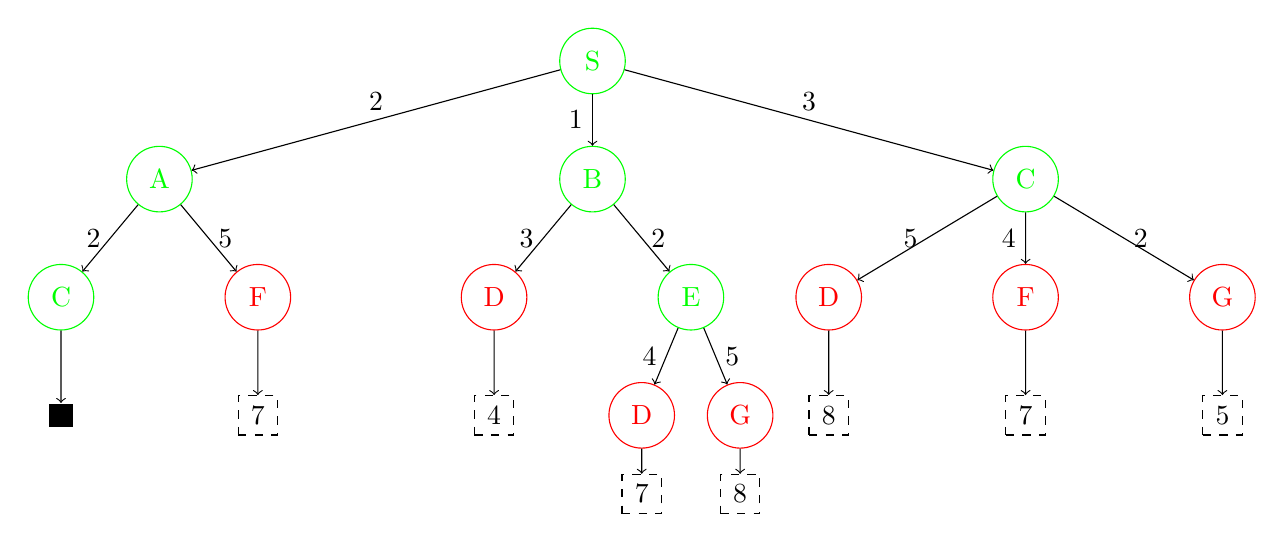
\begin{tikzpicture}[
            ->, 
            level/.style={level distance=1.5cm},
            level 1/.style={sibling distance=5.5cm},
            level 2/.style={sibling distance=2.5cm},
            level 3/.style={sibling distance=1.25cm},
            level 4/.style={sibling distance=1.75cm, level distance=1cm}
        ]
            \node[node_expanded] {S} 
                child { node[node_expanded]{A}
                    child { node[node_expanded]{C} 
                    child { node[node_leaf]{Z} }
                    edge from parent node[left]{2} }
                    child { node[node_non_expanded]{F} 
                    child { node[node_cost]{7} }
                    edge from parent node[right]{5} }
                edge from parent node[above]{2} }
                child { node[node_expanded]{B} 
                    child { node[node_non_expanded]{D}
                        child { node[node_cost]{4} }
                    edge from parent node[left]{3} }
                    child { node[node_expanded]{E} 
                        child { node[node_non_expanded]{D} 
                            child { node[node_cost]{7} }
                        edge from parent node[left]{4} }
                        child { node[node_non_expanded]{G} 
                            child { node[node_cost]{8} }
                        edge from parent node[right]{5} }
                    edge from parent node[right]{2} }
                edge from parent node[left]{1} }
                child { node[node_expanded]{C} 
                    child { node[node_non_expanded]{D} 
                    child { node[node_cost]{8} }
                    edge from parent node[left]{5} }
                    child { node[node_non_expanded]{F} 
                    child { node[node_cost]{7} }
                    edge from parent node[left]{4} }
                    child { node[node_non_expanded]{G} 
                    child { node[node_cost]{5} }
                    edge from parent node[right]{2} }
                edge from parent node[above]{3} }
            ;
        \end{tikzpicture}
    \end{center}
    \medskip
    \qquad \textit{Step 7.} We now try to expand node D since it is the cheapest. We have already expanded three of the children of D namely B, C and E. So only G remains.
    \smallskip
    \begin{center}
        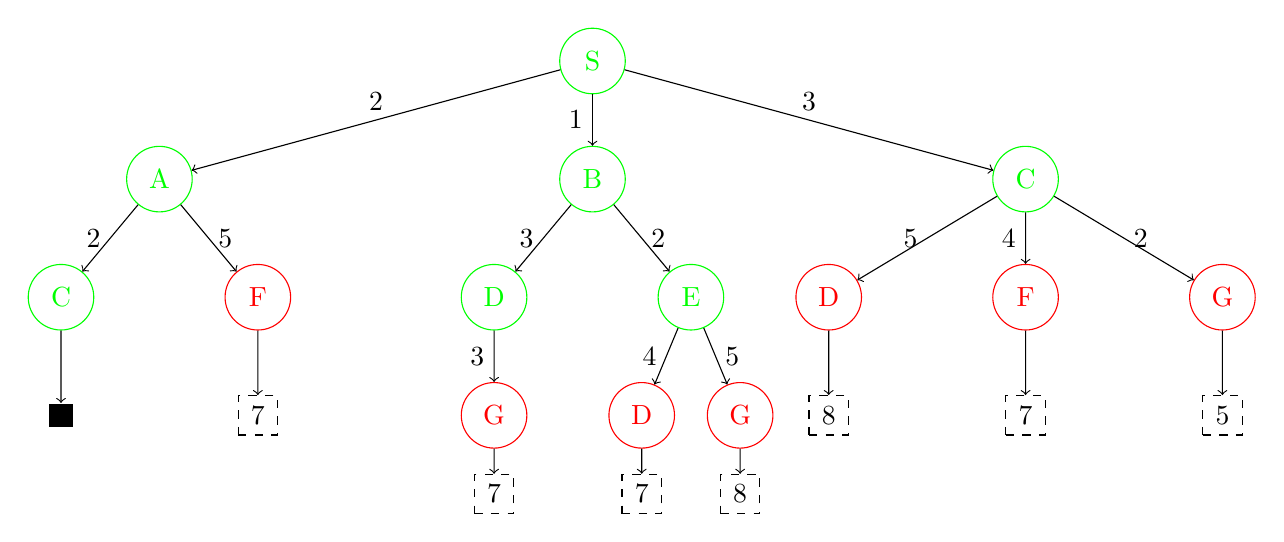
\begin{tikzpicture}[
            ->, 
            level/.style={level distance=1.5cm},
            level 1/.style={sibling distance=5.5cm},
            level 2/.style={sibling distance=2.5cm},
            level 3/.style={sibling distance=1.25cm},
            level 4/.style={sibling distance=1.75cm, level distance=1cm}
        ]
            \node[node_expanded] {S} 
                child { node[node_expanded]{A}
                    child { node[node_expanded]{C} 
                    child { node[node_leaf]{Z} }
                    edge from parent node[left]{2} }
                    child { node[node_non_expanded]{F} 
                    child { node[node_cost]{7} }
                    edge from parent node[right]{5} }
                edge from parent node[above]{2} }
                child { node[node_expanded]{B} 
                    child { node[node_expanded]{D}
                        child { node[node_non_expanded]{G} 
                            child { node[node_cost]{7} }
                        edge from parent node[left]{3} }
                    edge from parent node[left]{3} }
                    child { node[node_expanded]{E} 
                        child { node[node_non_expanded]{D} 
                            child { node[node_cost]{7} }
                        edge from parent node[left]{4} }
                        child { node[node_non_expanded]{G} 
                            child { node[node_cost]{8} }
                        edge from parent node[right]{5} }
                    edge from parent node[right]{2} }
                edge from parent node[left]{1} }
                child { node[node_expanded]{C} 
                    child { node[node_non_expanded]{D} 
                    child { node[node_cost]{8} }
                    edge from parent node[left]{5} }
                    child { node[node_non_expanded]{F} 
                    child { node[node_cost]{7} }
                    edge from parent node[left]{4} }
                    child { node[node_non_expanded]{G} 
                    child { node[node_cost]{5} }
                    edge from parent node[right]{2} }
                edge from parent node[above]{3} }
            ;
        \end{tikzpicture}
    \end{center}
    \pagebreak
    \qquad \textit{Step 8.} We now try to expand node G since it is the cheapest. Since G is our goal node, the search is over. The path returned by the uniform cost search is shown by the cyan line.
    \smallskip
    \begin{center}
        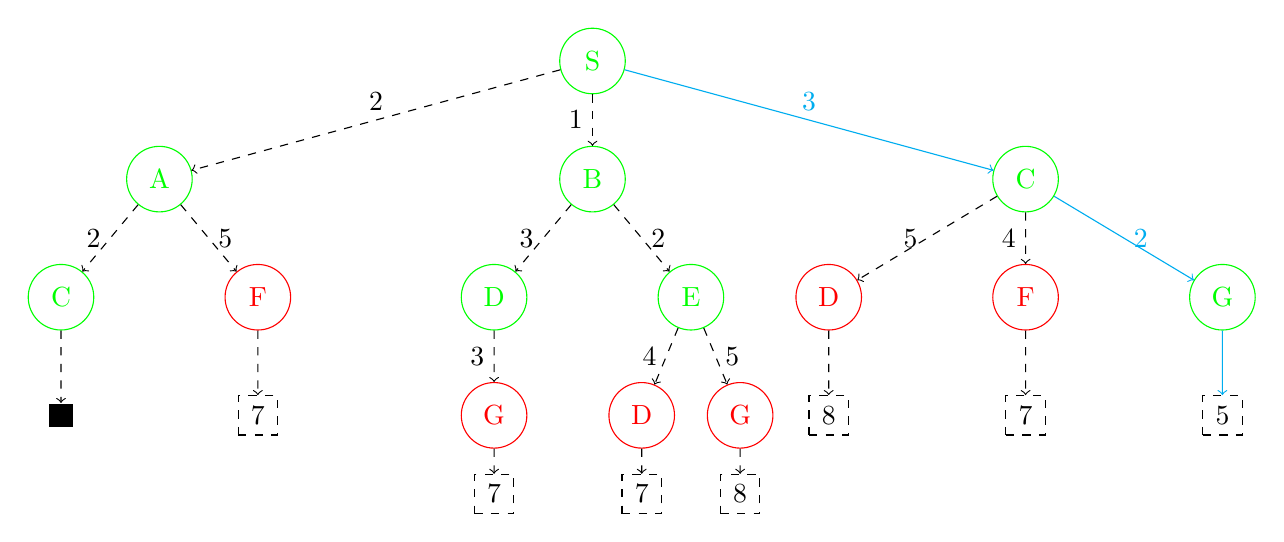
\begin{tikzpicture}[
            ->, 
            level/.style={level distance=1.5cm},
            level 1/.style={sibling distance=5.5cm},
            level 2/.style={sibling distance=2.5cm},
            level 3/.style={sibling distance=1.25cm},
            level 4/.style={sibling distance=1.75cm, level distance=1cm},
            every node/.style={solid}
        ]
            \node[node_expanded] {S} 
                child { node[node_expanded]{A} edge from parent [black, dashed]
                    child { node[node_expanded]{C}
                    child { node[node_leaf]{Z} }
                    edge from parent node[left]{2} }
                    child { node[node_non_expanded]{F} 
                    child { node[node_cost]{7} }
                    edge from parent node[right]{5} }
                edge from parent node[above]{2} }
                child { node[node_expanded]{B} edge from parent [black, dashed]
                    child { node[node_expanded]{D}
                        child { node[node_non_expanded]{G} 
                            child { node[node_cost]{7} }
                        edge from parent node[left]{3} }
                    edge from parent node[left]{3} }
                    child { node[node_expanded]{E} 
                        child { node[node_non_expanded]{D} 
                            child { node[node_cost]{7} }
                        edge from parent node[left]{4} }
                        child { node[node_non_expanded]{G} 
                            child { node[node_cost]{8} }
                        edge from parent node[right]{5} }
                    edge from parent node[right]{2} }
                edge from parent node[left]{1} }
                child { node[node_expanded]{C} edge from parent [cyan]
                    child { node[node_non_expanded]{D} edge from parent [black, dashed]
                    child { node[node_cost]{8} }
                    edge from parent node[left]{5} }
                    child { node[node_non_expanded]{F} edge from parent [black, dashed]
                    child { node[node_cost]{7} }
                    edge from parent node[left]{4} }
                    child { node[node_expanded]{G} edge from parent [cyan]
                    child { node[node_cost]{5} }
                    edge from parent node[right]{2} }
                edge from parent node[above]{3} }
            ;
        \end{tikzpicture}
        $$ \Rightarrow Cost = 5 $$
    \end{center}
    \bigskip
    To summarize, the paths and the costs returned by different search methods are listed below.
    \medskip
    \begin{center}
        \scalebox{1.25}[1.28]{
            \begin{tabular}{|c||c||c|}
                \hline
                Method & Path & Cost \\
                \hline
                BFS & $ S \rightarrow C \rightarrow G $ & $ 5 $ \\
                \hline
                DFS & $ S \rightarrow A \rightarrow C \rightarrow D \rightarrow B \rightarrow E \rightarrow G $ & $ 19 $ \\
                \hline
                IDS & $ S \rightarrow A \rightarrow C \rightarrow G $ & $ 6 $ \\
                \hline
                UCS & $ S \rightarrow C \rightarrow G $ & $ 5 $ \\
                \hline
            \end{tabular}
        }
    \end{center}
\end{document}
